\section{Nomenclature}

To establish a comon language, in the following some of the nomenclature used at Revolve NTNU is explained. \\

A lot of the following discussion will deal with two main frames of references. One is the "base link" frame, sometimes referred to as the "body" frame. It is situated in the center of gravity (CG) of the car, with it's x-axis going in the longitudinal, the forward, direction of the car, it's z-axis upwards away from the ground and it's y-axis going in the left lateral direction, i.e. completing a right hand frame with the x- and the z-axis. This is illustrated in figure \ref{Fig:BodyFrame}. \\ 

The other main frame is the "map" frame. It starts with the same position and orientation as the body frame when the car starts, put then remains fixed in the same pose relative to the earth fixed frame until the system is reset. It is illustrated in figure \ref{Fig:MapAndBodyFrames}. \\

Between these two frames lives another one; the odometry frame. It is in this frame that the autonomous system makes its first estimate of the cars pose relative to the map frame, using only the estimations coming out of the state estimation node. This is however subject to drift and errors, and over time will not be the true pose of the car. This is therefore corrected by the SLAM node, outputting the transformation between map and odometry frames. This is possible since SLAM is supposed to be "grounded" to the real world by direct measurements of the landmarks in the map it has built. More on this later. The relationship between the map, odometry and body frames are illustrated in figure \ref{Fig:MapOdomAndBodyFrames}. \\ 

\begin{figure}
    \centering
    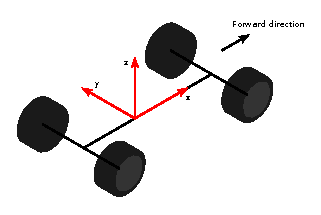
\includegraphics[width=0.5\linewidth]{0_Images/2_Introduction/BaseLinkFrame.eps}
    \captionof{figure}{The "base link" or "body" frame.}
    \label{Fig:BodyFrame}
\end{figure}

\begin{figure}
    \centering
    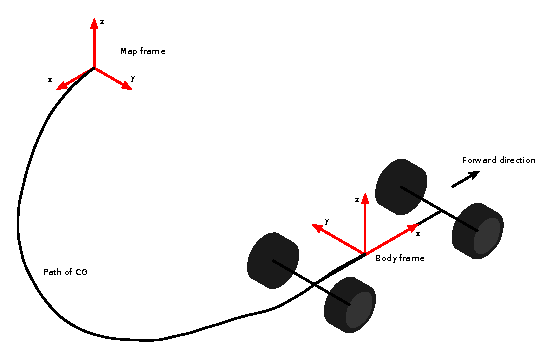
\includegraphics[width=0.5\linewidth]{0_Images/2_Introduction/MapAndBodyFrames.eps}
    \captionof{figure}{The map and body frames.}
    \label{Fig:MapAndBodyFrames}
\end{figure}

\begin{figure}
    \centering
    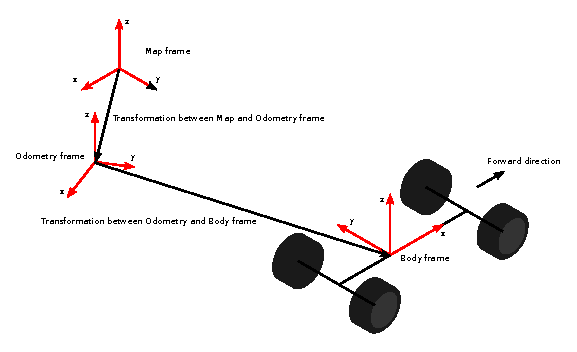
\includegraphics[width=0.5\linewidth]{0_Images/2_Introduction/MapOdomAndBodyFrames.eps}
    \captionof{figure}{The relationship between the map, odometry and body frames.}
    \label{Fig:MapOdomAndBodyFrames}
\end{figure}

Before leaving the realm of coordinate frames, one more must be mentioned. In the center of each wheel is defined a reference frame, here called the wheel frame. When the wheel is pointed straight ahead it has the same orientation as the body frame. This is illustrated in figure \ref{Fig:WheelFrame}. This frame will be important for talking about summing the forces from each wheel into one force and one torque on the CG. \\

Furthermore it is benefitial to name a few of the components of the race car. The main hoop is the bended rod around the drivers head that saves him or her from being crushed by the car if it should ever roll over. The snout is the rounded tip of the front of the car. The track of the car referes to the distance between the front and rear wheels along the x-axis, while the wheelbase refers to the distance between the right and left wheels along the y axis. These terms are illustrated in figure \ref{Fig:NameOfCarParts}.

\begin{figure}
    \centering
    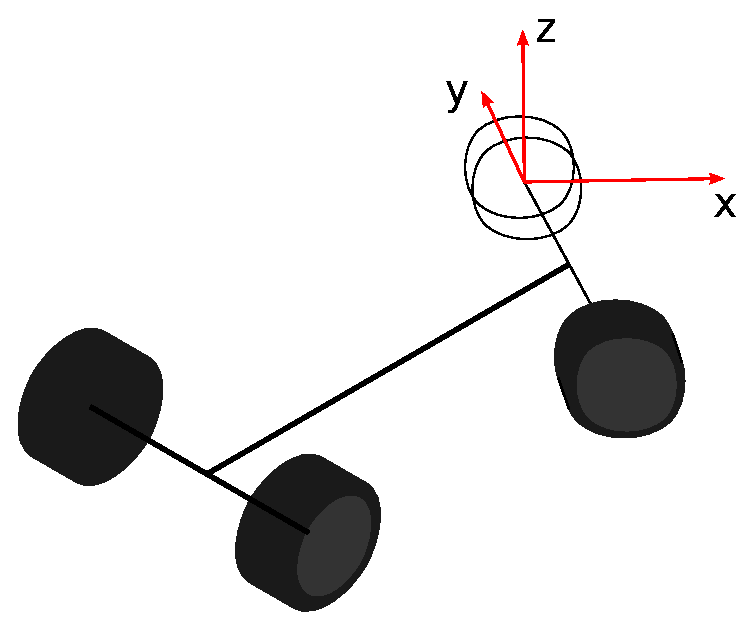
\includegraphics[width=0.5\linewidth]{0_Images/2_Introduction/WheelFrame.eps}
    \captionof{figure}{Front left wheel frame. There are similar ones in the other three wheels.}
    \label{Fig:WheelFrame}
\end{figure}


\begin{figure}
    \centering
    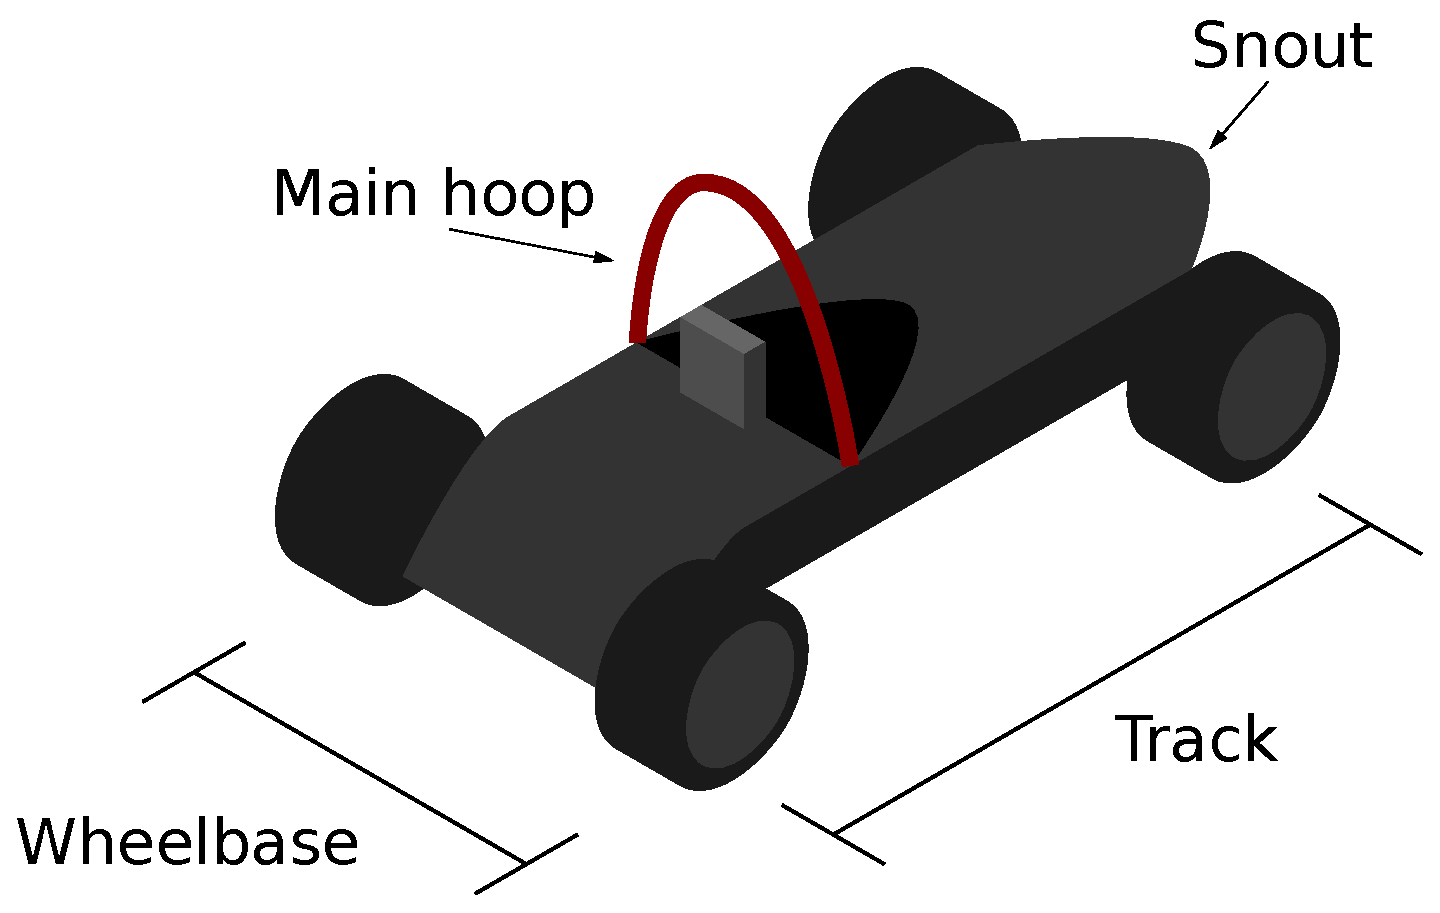
\includegraphics[width=0.5\linewidth]{0_Images/2_Introduction/NameOfCarParts.eps}
    \captionof{figure}{Simple model of the car with names of some parts, along with illustrations of track and wheelbase.}
    \label{Fig:NameOfCarParts}
\end{figure}
